\lettrine[findent=0.3em, nindent=0em]{\textbf{P}}{ower consumption} and heat
dissipation are of great importance. Power translates to energy, and energy to
hours of battery life and to electricity bills. Temperature, on the other hand,
is one of the major causes of permanent damage \cite{jedec}, which necessitates
adequate cooling equipment and, hence, escalates product expenses
\cite{chaudhry2015}. The situation is deteriorated further by the
power-temperature interplay: higher power leads to higher temperature, and
higher temperature to higher power \cite{liu2007}. Therefore, accounting for
power and temperature is key to achieving effectiveness, efficiency, and
robustness.

Our work is to assist researchers who are concerned with power and temperature
in one specific but rather broad context: the development of data-driven power-
and temperature-aware solutions for computer systems where \emph{data-driven}
refers to the usage of algorithms that learn from data \cite{bishop2006}. To
this end, we develop a toolchain for fast synthesis of realistic power and
temperature profiles, which is motivated as follows.

The power and temperature characteristics of a computer system are difficult to
describe mathematically or algorithmically. Modern computer systems are complex,
and many aspects are inherently uncertain to the designer due to such phenomena
as process variation \cite{chandrakasan2000}, aging \cite{coskun2006}, and
varying workload. The concern is particularly difficult to address from a
theoretical standpoint; it can be better dealt with taking a more pragmatic
approach, namely, making use of runtime data. Assuming that the system provides
mechanisms for profiling and monitoring, direct or indirect power and
temperature readings are an invaluable source of information for making
proactive power- and temperature-aware decisions \cite{chaudhry2015,
coskun2008}.

\begin{figure}
  \centering
  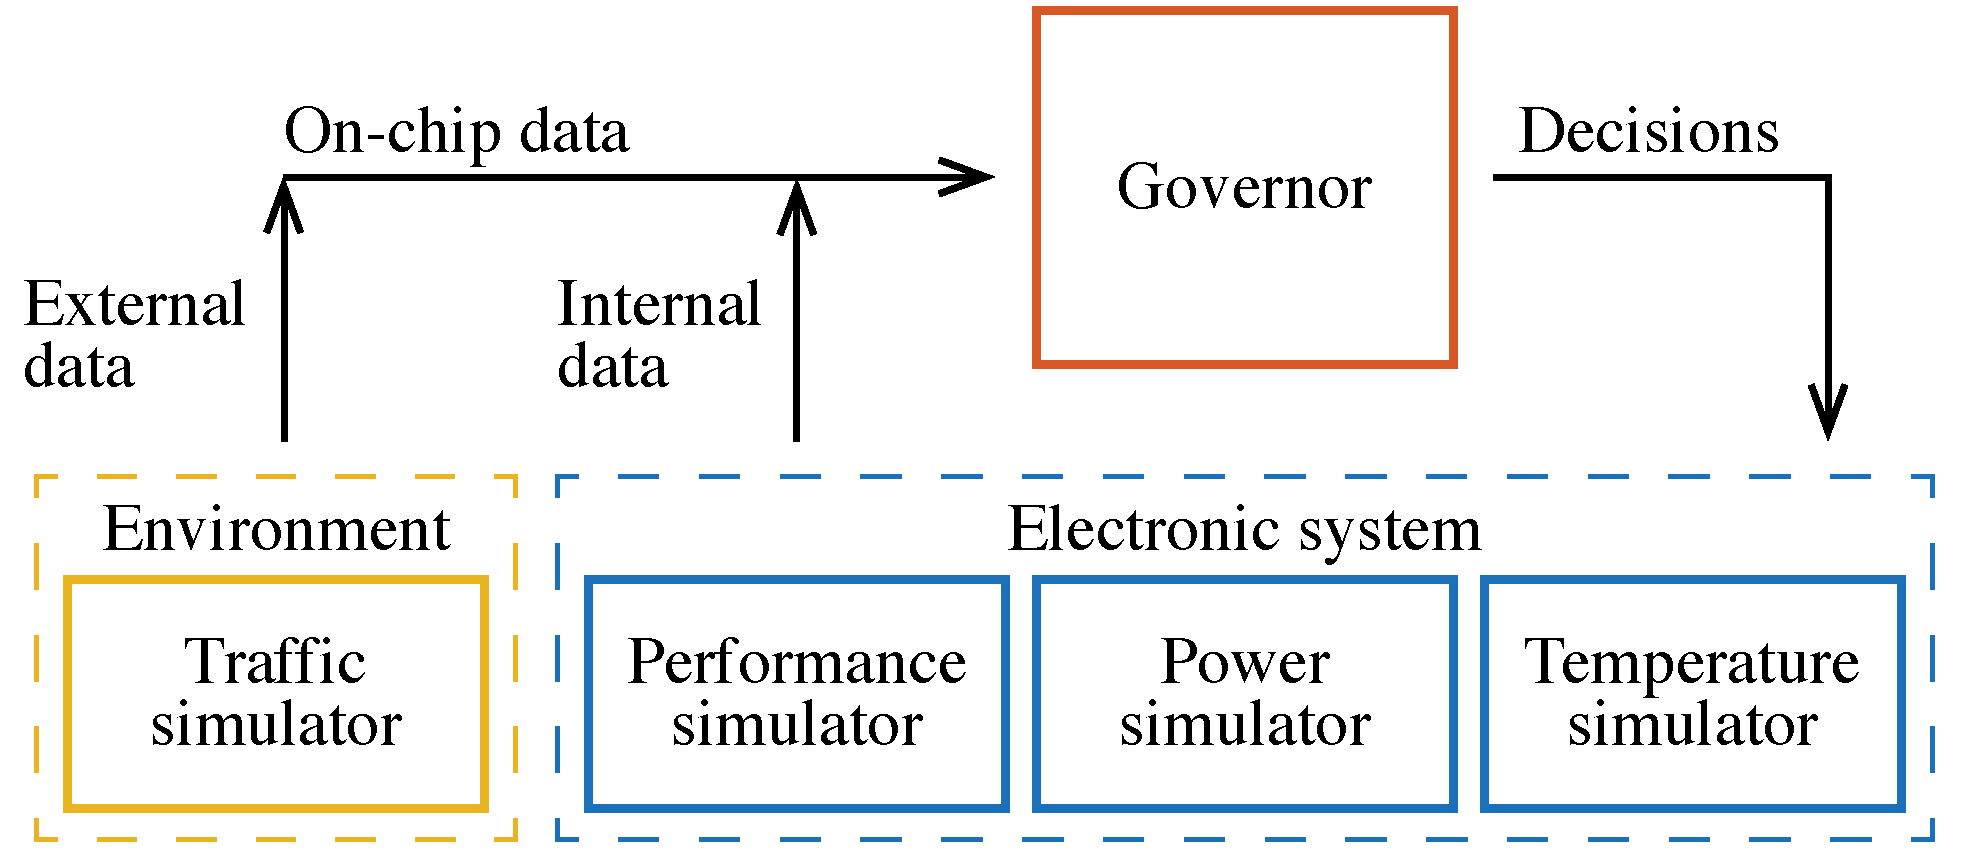
\includegraphics[width=1.0\columnwidth]{include/assets/figures/development.pdf}

  \caption{An experimental setup for developing management strategies
  (governors). \emph{Online data} refers to the data available on the chip
  regardless of their origin. The right dashed box should be understood at a
  single module, and the corresponding arrows should be treated accordingly.}

  \flab{development}
\end{figure}

Acting proactively requires forecasting the future by learning from the past,
which is typically accomplished by virtue of machine learning \cite{bishop2006}.
Regardless of the learning technique utilized, the technique requires data to
learn from. Real data are rarely available in large enough quantities. The
target platform might not be at one's disposal or might not be an appropriate
place for early experimentation, which is common in research. Therefore, a
research environment is typically composed of a number of computer simulators as
they constitute a feasible alternative source of the needed data. An
illustrative example is given in \fref{development}, which depicts a potential
environment for developing a resource manager for a computer system.

Computer simulators, however, fall short when it comes to complex systems: it
might take days for a state-of-the-art simulator to simulate a short, in
wall-clock time, program. This scheme is not affordable for designing
data-driven solutions as they require many simulations with potentially large
payloads.

To summarize, real data are rarely and sparingly available, and simulation data
are prohibitively time consuming to obtain, which hampers the development of
data-driven solutions. The need for alternative sources of high-quality data is
prominent, which brings us to the goal of this work: our objective is to provide
such a source for the case of power and temperature.

It is well understood that the solution being developed will eventually face
real data, and, therefore, it should be tested and, if it is needed, calibrated
in a stage environment prior to deploying the solution to a production
environment. The synthetic data that we generate can substantially speed up this
process due to the flexibility and fast feedback that they provided. In
particular, one can filter out inadequate ideas at early stages and focus solely
on those that are viable.

The remainder of the paper is organized as follows. In \sref{literature}, we
elaborate on the related work and summarize our contribution. The addressed
problem is formalized in \sref{problem}. The methodology that we follow and our
toolchain are presented in \sref{methodology} and \sref{toolchain},
respectively. The experimental results are given in \sref{result}. Section
\ref{sec:conclusion} concludes the paper.
